
\noindent\begin{minipage}{\textwidth}
    \begin{table}[H]
        \centering
        \caption{Hiperparâmetros e Resultados do Melhor Modelo - convnext\_v12\_BR\_opt\_aug}
        \vspace{0.2cm}
        \resizebox{\textwidth}{!}{%
            \begin{tabular}{ll | lrrr}
                \hline
                \multicolumn{2}{c|}{\textbf{Hiperparâmetros}} & \multicolumn{4}{c}{\textbf{Métricas por Classe}} \\ \hline
                \textbf{Parâmetro} & \textbf{Valor} & \textbf{Classe} & \textbf{Precisão} & \textbf{Recall} & \textbf{F1-Score} \\ \hline
    Agendador (\$T\_0\$) & 6 & 31.2 & 0,4870 & 0,4234 & 0,4530 \\ 
Agendador de LR & CosineAnnealingWarmRestarts & 31.3 & 0,2242 & 0,4043 & 0,2884 \\ 
Architecture & convnext\_tiny & 31.4 & 0,2941 & 0,4386 & 0,3521 \\ 
Batch Size & 32 & 32.3 & 0,3333 & 0,0952 & 0,1481 \\ 
Data Augmentation & False & 32.4 & 0,0476 & 0,0278 & 0,0351 \\ 
Decaimento de Peso (WD) & 0,0338 & 33.3 & 0,2618 & 0,2824 & 0,2717 \\ 
Dropout & 0,2943 & 41.4 & 0,2500 & 0,0426 & 0,0727 \\ 
Função de Perda & CrossEntropyLoss & 41.5 & 0,5652 & 0,3023 & 0,3939 \\ 
Hidden Units & 512 & 42.4 & 0,1556 & 0,1148 & 0,1321 \\ 
Label Smoothing & 0,1758 & 44.4 & 0,3333 & 0,0625 & 0,1053 \\ 
\cline{3-6} 
Otimizador & AdamW & \textbf{Média (Macro)} & 0,4513 & 0,2082 & 0,2136 \\ 
Taxa de Aprendizado (LR) & 1,58e-04 & \textbf{MCC} & \multicolumn{3}{c}{0,1793} \\ 
Unfreeze Layers & 5 &  & & &  \\ 
            \hline
            \end{tabular}%
        }
    \end{table}

    \begin{figure}[H]
        \centering
        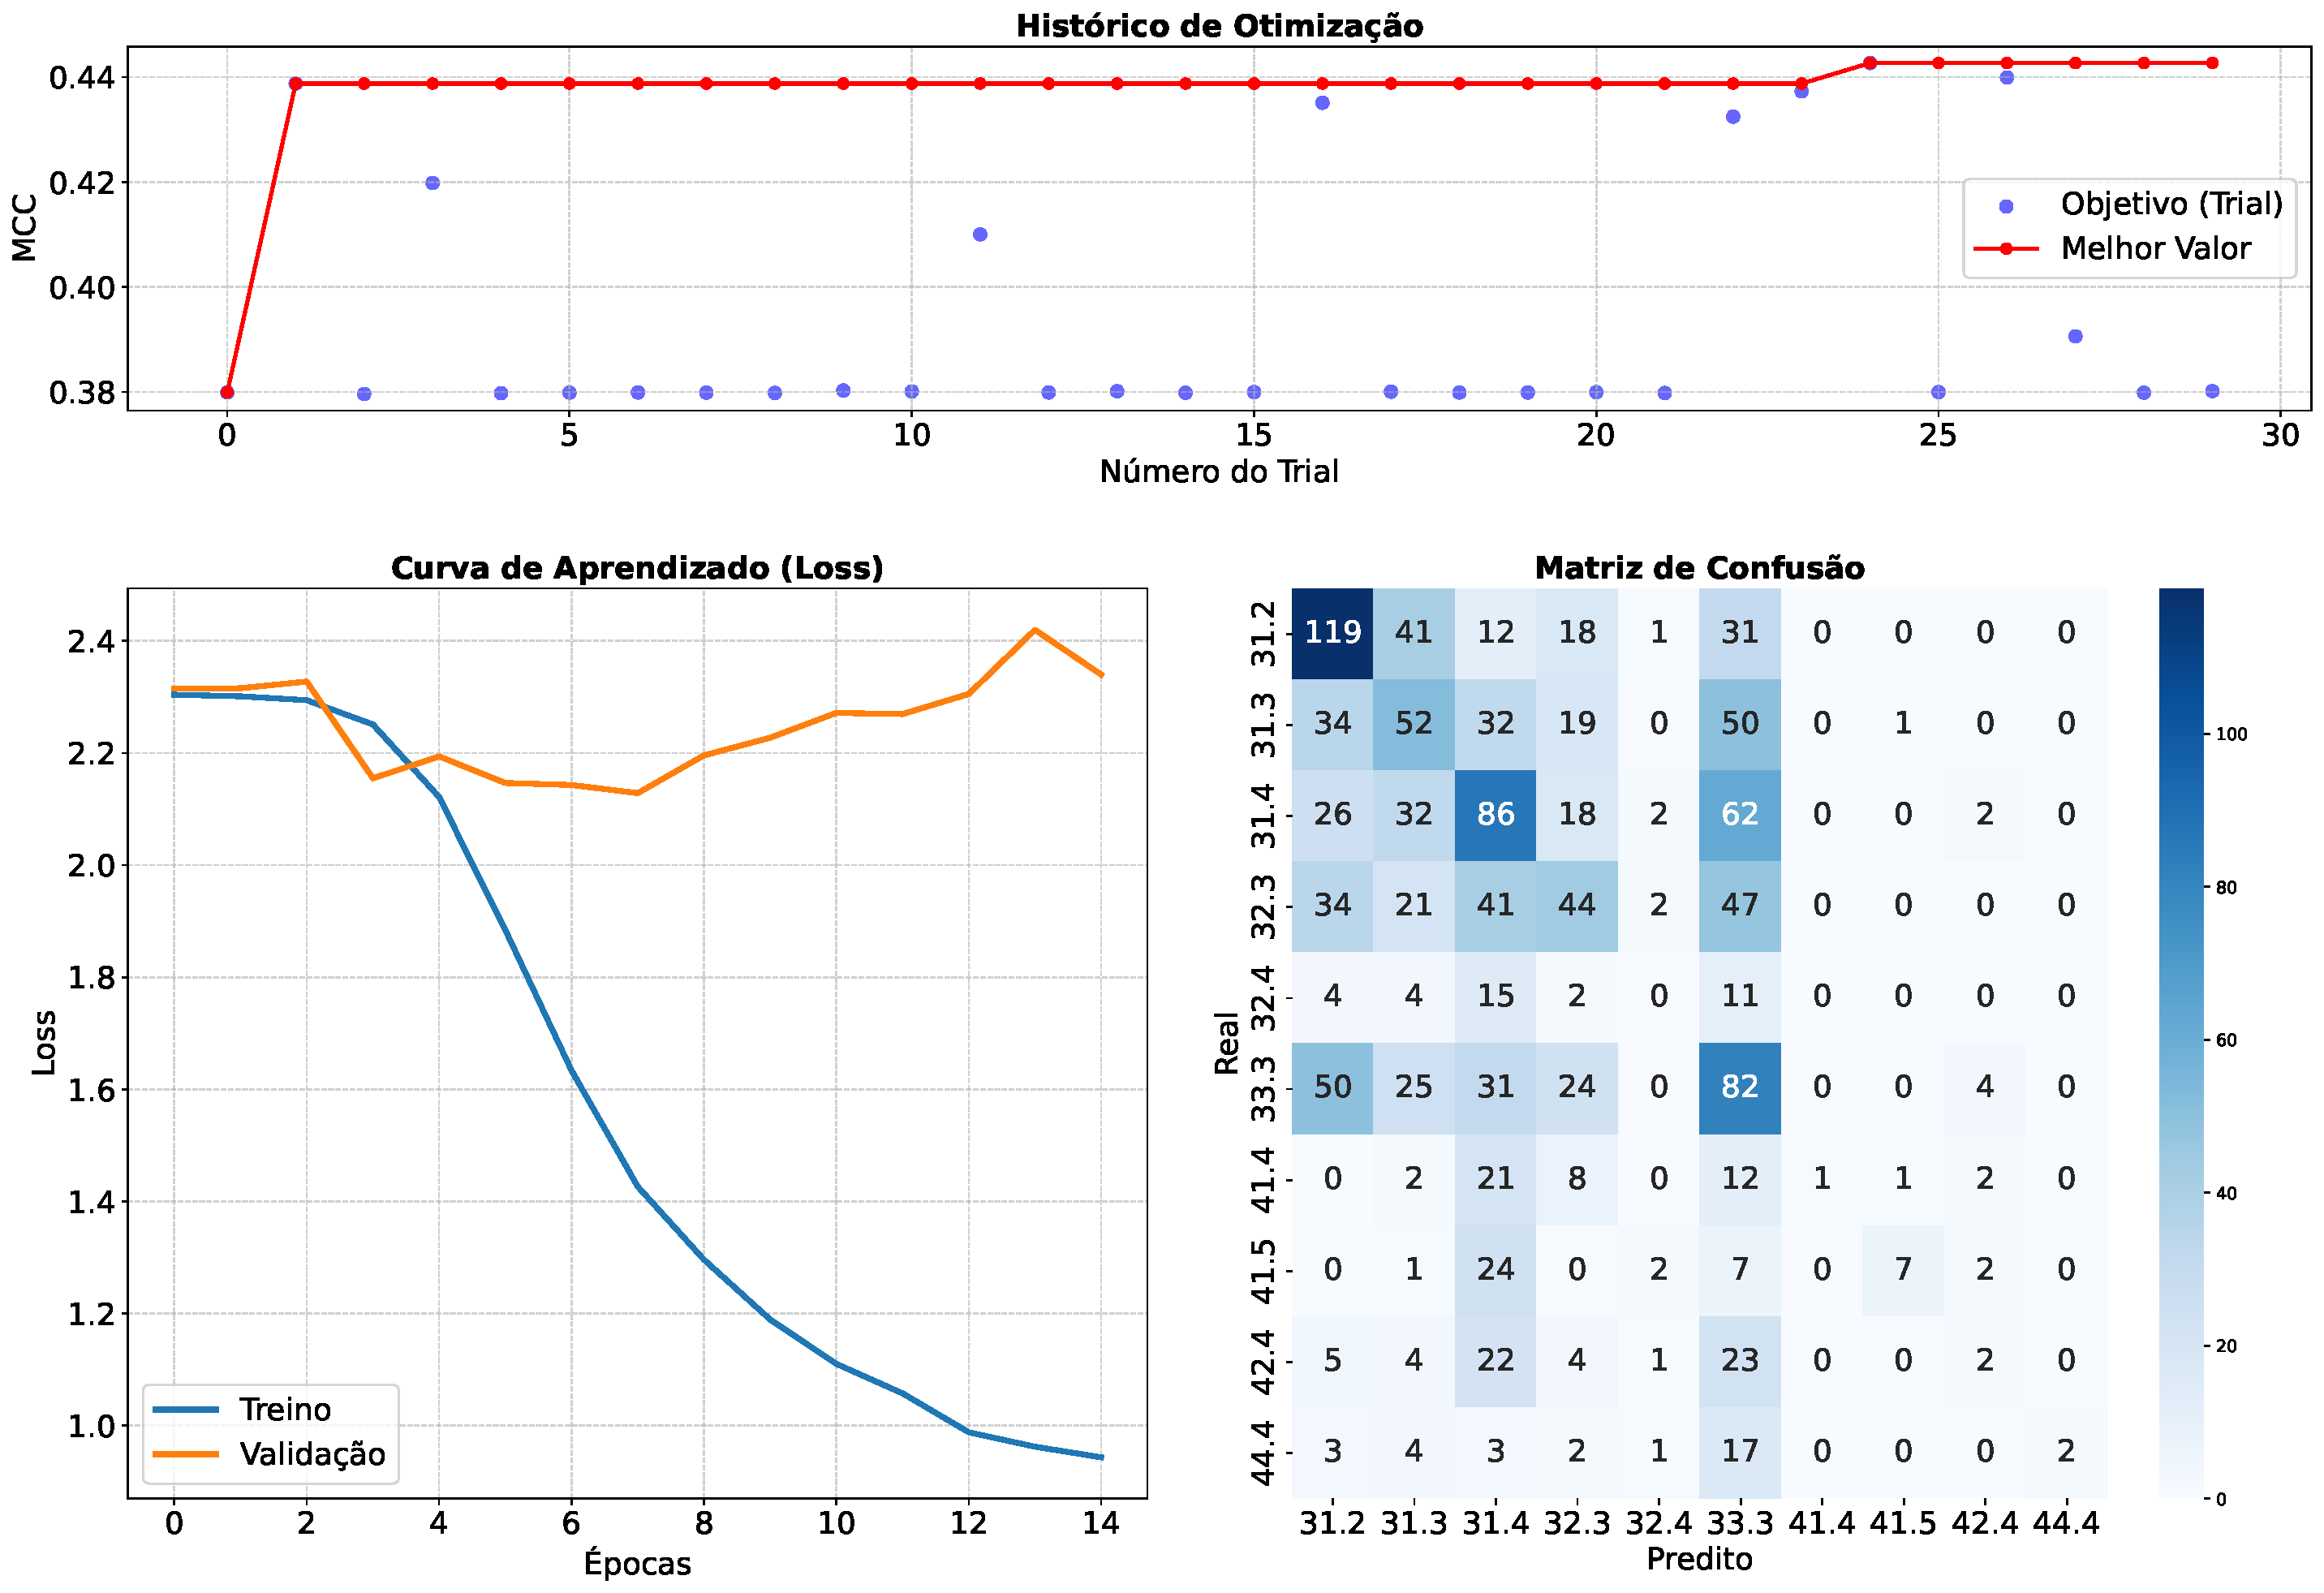
\includegraphics[width=0.85\textwidth]{tex/appendix/experiments/convnext_v12_BR_opt_aug/dashboard_consolidado.pdf}
        \caption{Histórico de Otimização, Curvas de Aprendizado e Matriz de Confusão - convnext\_v12\_BR\_opt\_aug}
    \end{figure}
\end{minipage}
\clearpage
